\chapter{Hipótesis}
La hipótesis es la respuesta al problema de la investigación. La hipótesis, al igual que el problema y los objetivos se describen en tiempo presente. Siempre debemos intentar hacer que las relaciones sean positivas (Directamente), no negativas (Inversamente)

    \begin{figure}[H]
        \centering
        %\isPreprints{\centering}{} % Only used for preprints
        \caption{Hipótesis
        \label{fig-modelo-hipótesis}}    
                
        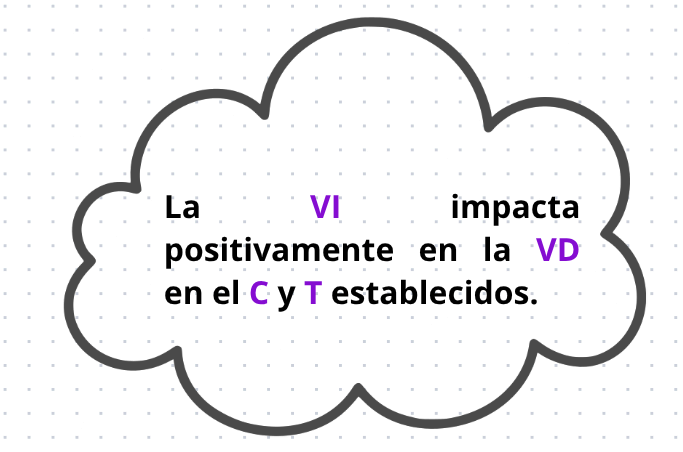
\includegraphics[width=7.0 cm]{src/imgs/hipótesis.png}

        \vspace{0.1cm}
        % \small EN CASO DE SER BAJO ELABORACIÓN PROPIA, NO HACE FALTA AGREGAR LA NOTA
    \end{figure}

    \begin{figure}[H]
        \centering
        %\isPreprints{\centering}{} % Only used for preprints
        \caption{Relación Inversa hasta la Hipótesis
        \label{fig-relacion-inversa-hipótesis}}    
                
        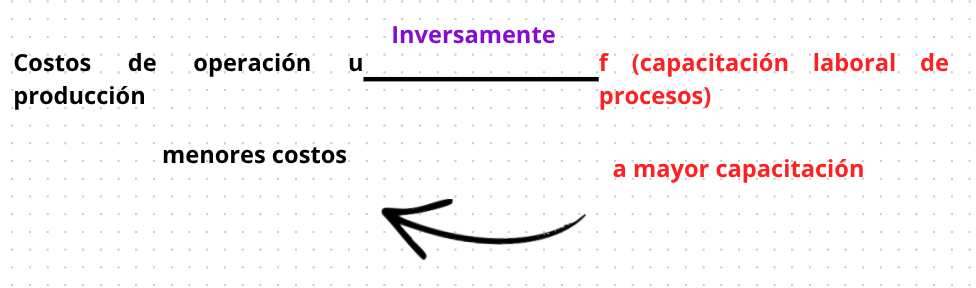
\includegraphics[width=11.0 cm]{src/imgs/relacion-inversa-hipotesis.png}

        \vspace{0.1cm}
        % \small EN CASO DE SER BAJO ELABORACIÓN PROPIA, NO HACE FALTA AGREGAR LA NOTA
    \end{figure}

\section{Hipótesis General}
    \begin{sectext}
        Lorem ipsum dolor sit amet consectetur adipisicing elit.
    \end{sectext}

\section{Hipótesis Específicas}
    \begin{sectext}
        \begin{itemize}
            \item Lorem ipsum dolor sit amet consectetur adipisicing elit.
            \item Lorem ipsum dolor sit amet consectetur adipisicing elit.
        \end{itemize}
    \end{sectext}